\chapter{Architecture générale du modèle}
\label{ch:architecture}

\section{Ce que le modèle représente}

Le modèle est une représentation chiffrée de l'économie française, construite pour répondre à une question précise :
\emph{si l'on modifie un impôt, une dépense, une prestation ou une règle, que se passe-t-il pour l'activité, l'emploi,
les prix, les revenus des ménages, les finances publiques et la répartition des niveaux de vie, et à quel horizon ?}
Il ne cherche pas à prévoir l'avenir : il compare deux avenirs possibles, l'un sans la mesure (la \emph{référence}),
l'autre avec. C'est ce que les économistes appellent une \emph{variante}.

Il appartient à la famille des \emph{modèles macro-économétriques semi-structurels} utilisés par l'administration
française (Mésange à l'Insee et à la direction générale du Trésor, FR-BDF à la Banque de France), auxquels il emprunte
la logique : des comportements estimés sur l'histoire (consommer, investir, embaucher, fixer les prix et les salaires,
importer, exporter), insérés dans une comptabilité nationale cohérente qui garantit que chaque euro dépensé par un agent
est reçu par un autre. Il s'en distingue par trois choix :
\begin{enumerate}
  \item il est entièrement construit sur des \textbf{données ouvertes} et son code est public ;
  \item il est relié à une \textbf{microsimulation des ménages} (OpenFisca-France appliqué à un échantillon de ménages
  réels du recensement), qui calcule impôts et prestations ménage par ménage et permet de mesurer la pauvreté et les
  inégalités ;
  \item il décrit l'appareil productif en \textbf{64 produits et 25 branches marchandes}, ce qui permet de suivre la
  propagation d'un choc d'énergie ou d'une politique industrielle d'une branche à l'autre.
\end{enumerate}

\begin{encadre}{Encadré 1.1 — Qu'est-ce qu'un modèle, et que peut-on en attendre ?}
Un modèle est un ensemble d'équations qui relient des grandeurs économiques entre elles. Certaines équations sont des
\textbf{identités comptables}, vraies par définition : le PIB est égal à la somme des valeurs ajoutées, la dette de fin
d'année est égale à la dette de début d'année plus le déficit. D'autres sont des \textbf{équations de comportement} : elles
décrivent comment, \emph{en moyenne dans le passé}, les ménages ont ajusté leur consommation à leur revenu, ou les
entreprises leurs embauches à leur production. Ces relations sont estimées statistiquement ; elles comportent une marge
d'erreur, et rien ne garantit qu'elles resteront valables si l'on change profondément les règles du jeu (c'est la
« critique de Lucas »). Enfin, certaines relations sont des \textbf{hypothèses} faute de données : le modèle les
signale comme telles.

Un modèle est donc un instrument de \emph{raisonnement chiffré} : il rend explicites des chaînes de causalité et en
donne des ordres de grandeur. Il ne remplace ni l'évaluation après coup des politiques, ni le débat sur les choix
de société.
\end{encadre}

\section{Les acteurs et leurs échanges}

La figure~\ref{fig:architecture} présente les grands acteurs (au sens de la comptabilité nationale : les \emph{secteurs
institutionnels}) et les flux qui les relient.

\begin{figure}[htbp]
\centering
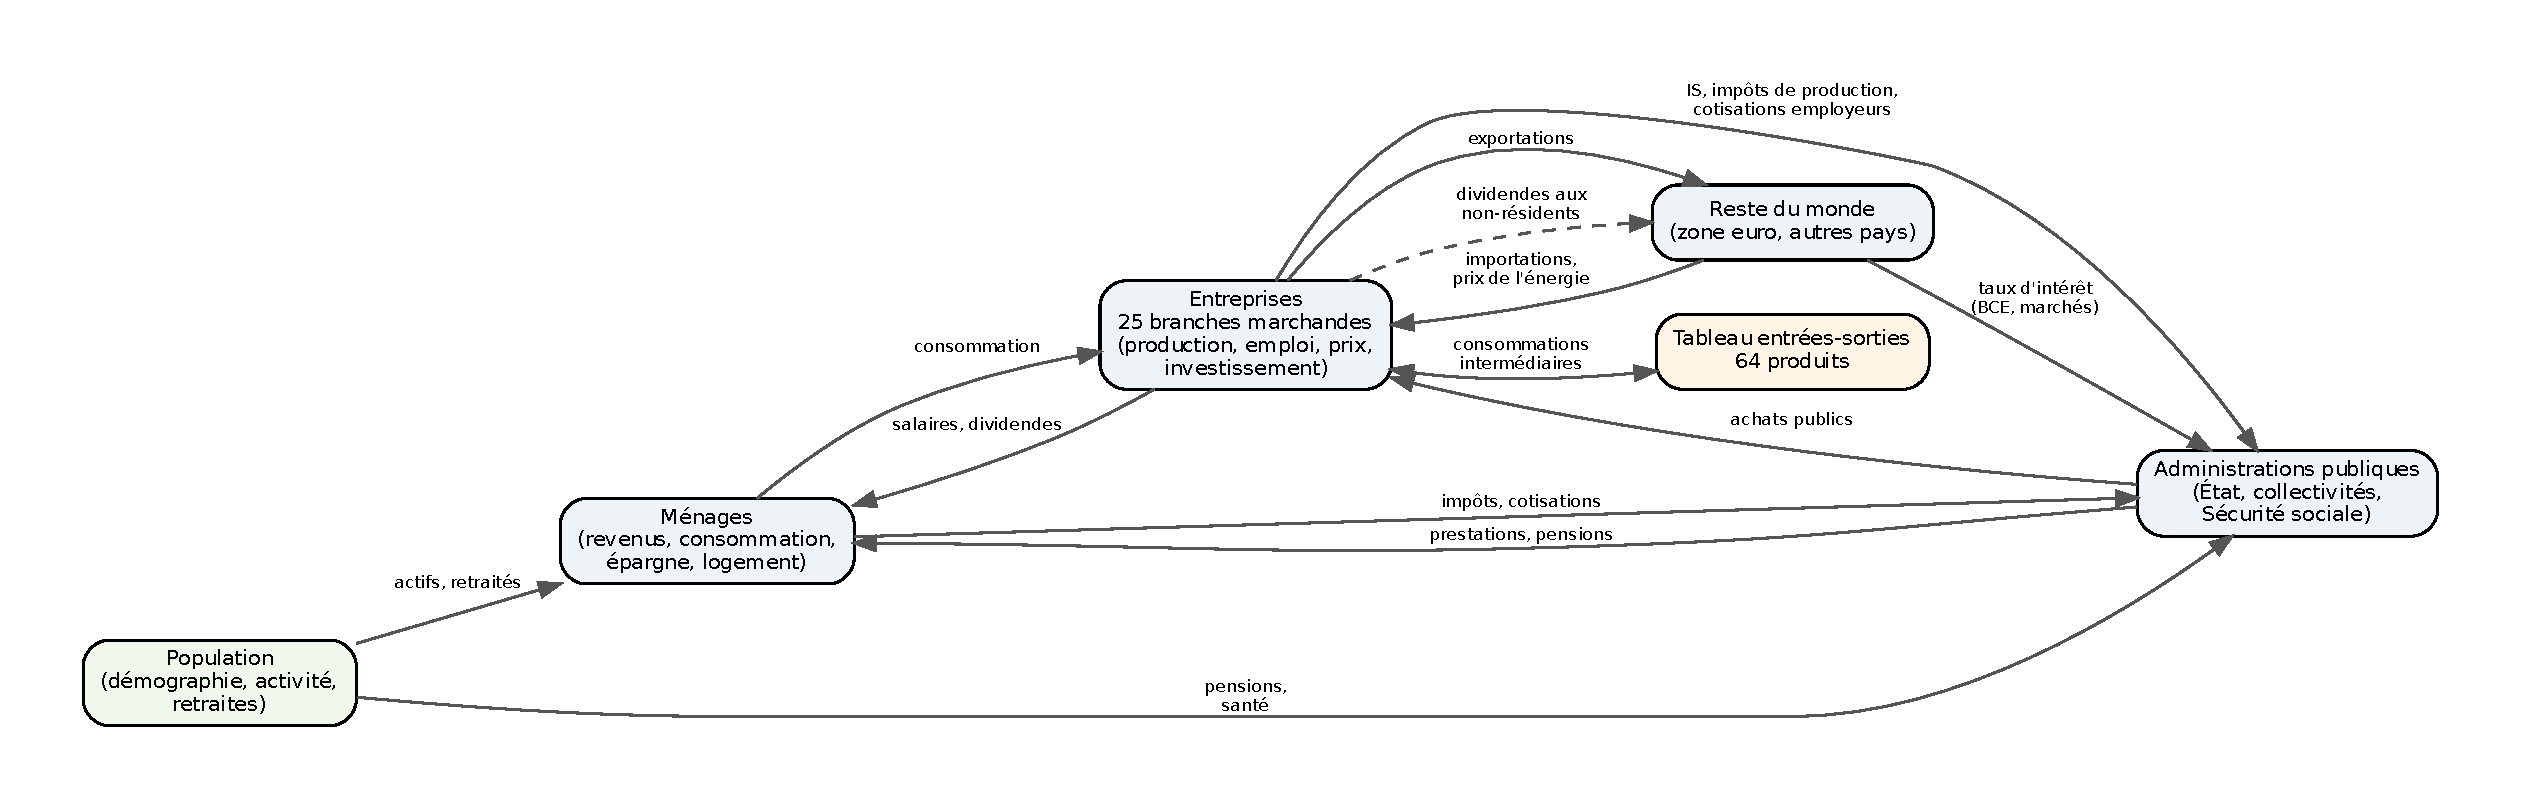
\includegraphics[width=\linewidth]{architecture.pdf}
\caption{Architecture du modèle : secteurs institutionnels et principaux flux. Les flèches pleines sont des flux
monétaires représentés par des équations ; la flèche pointillée (dividendes versés aux non-résidents) n'est active que
pour les mesures qui modifient les profits des entreprises. Le tableau entrées-sorties décrit les échanges entre
produits.}
\label{fig:architecture}
\end{figure}

\begin{description}[style=nextline,leftmargin=1.2em]
\item[Les ménages] perçoivent des salaires, des revenus d'indépendants, des revenus du patrimoine (intérêts,
dividendes, loyers) et des prestations sociales (pensions, allocations, minima sociaux) ; ils paient des impôts
(impôt sur le revenu, CSG) et des cotisations. Ce qui reste est leur \emph{revenu disponible brut} (RDB). Ils en
consomment la plus grande partie, investissent dans le logement et épargnent le reste.
\item[Les entreprises] sont décrites par 25 branches marchandes (agriculture, 15 branches industrielles, énergie,
construction, commerce, transport, hébergement-restauration, information-communication, finance, services aux
entreprises, autres services). Chaque branche produit, emploie, fixe ses prix, investit. La production non marchande
(administration, enseignement, santé publique) et l'immobilier forment une branche à part, dont le volume suit la
dépense publique.
\item[Les administrations publiques] (État, collectivités locales, sécurité sociale, organismes sociaux) prélèvent
impôts et cotisations, versent rémunérations, achats, prestations et intérêts, et s'endettent quand les dépenses
excèdent les recettes. Le modèle ne distingue pas les sous-secteurs : les organismes de sécurité sociale (retraites,
assurance maladie, chômage) sont consolidés avec l'État et les collectivités, comme dans la notification du déficit
au sens de Maastricht.
\item[Le reste du monde] achète nos exportations, nous vend des importations (dont toute l'énergie fossile), fixe les
prix mondiaux, et — par la Banque centrale européenne et les marchés — les taux d'intérêt. Une part des dividendes
des entreprises françaises lui revient.
\item[La population] (démographie par âge et par sexe, activité, retraite) détermine le nombre d'actifs et de
retraités, donc l'offre de travail et la masse des pensions.
\end{description}

\paragraph{Flux énergétiques, matériels et logistiques.}
Le modèle ne suit pas de flux physiques (tonnes, kilowattheures) : il représente l'énergie et les matières par leurs
\emph{flux monétaires} dans le tableau entrées-sorties. Trois produits énergétiques sont distincts : industries
extractives (pétrole brut, gaz, minerais), raffinage, électricité-gaz-vapeur. Une hausse du prix de l'énergie importée
se propage aux coûts de toutes les branches selon leur consommation directe et indirecte d'énergie. La logistique
(transport, entreposage, commerce) est une branche comme une autre ; ses marges sont comptées dans la valeur ajoutée
française des produits importés. Il n'y a ni substitution entre énergies, ni contrainte physique de ressources :
\emph{c'est une limite importante} pour les questions de transition énergétique (chapitre~\ref{ch:audit}).

\section{Les modules}

Le modèle est organisé en modules, numérotés dans l'ordre de leur construction (tableau~\ref{tab:modules}). Le
chapitre~\ref{ch:sousmodeles} les documente un par un.

\begin{table}[htbp]
\centering\small
\caption{Les modules du modèle et leur rôle.}
\label{tab:modules}
\begin{tabularx}{\linewidth}{@{}l>{\raggedright\arraybackslash}p{3.6cm}L@{}}
\toprule
Module & Objet & Contenu principal \\
\midrule
M1 & Démographie & Population par âge simple et sexe, 2026-2070 (méthode et hypothèses de l'Insee) \\
M3 & Cadre comptable & Comptes non financiers de la France par secteur, 2019-2025 ; identités vérifiées \\
M4 & Population de ménages & 164\,000 ménages réels du recensement 2022, revenus calés sur la DGFiP, impôts et prestations par OpenFisca \\
M5 & Bloc productif & Tableau entrées-sorties 64 produits, modèle de prix et de quantités \\
M7 & Comportements & 12 équations estimées sur 1997-2019 (emploi, prix, salaires, investissement, consommation, logement, commerce extérieur, transmission des prix importés, revenus du patrimoine) \\
M8 & Modèle bouclé & Résolution annuelle simultanée de toutes les équations ; finances publiques ; trajectoire de référence \\
M9 & Activité des seniors et retraites & Taux d'activité de 55 à 74 ans selon l'âge légal ; pensions par génération \\
M10 & Couplage micro-macro & Passage des résultats ménage par ménage (OpenFisca) au modèle bouclé ; pauvreté, inégalités \\
M11 & Europe & Règle de taux de la BCE, taux longs français, prime de risque, demande des partenaires \\
M12 & Incertitude & Tirages Monte-Carlo des coefficients estimés et des paramètres calibrés \\
M13 & Hauts revenus et patrimoines & Réactions d'optimisation et de mobilité (élasticités de la littérature) \\
M14 & Hétérogénéité & Propension à consommer par décile, distribution des profits, dividendes aux non-résidents \\
\midrule
Simulateur & Catalogue de mesures & 41 curseurs traduits en entrées des modules ; mise en œuvre à partir de 2028 \\
\bottomrule
\end{tabularx}
\end{table}

Le numéro M2 (prévu pour une population synthétique dynamique) et M6 (prévu pour un bloc financier complet) n'ont pas
été construits : ils figurent dans le plan initial mais ont été remplacés par M4 (population statique réelle) et par
la seule dette publique. Le modèle n'a donc \textbf{pas de bilan financier complet} des agents (section~\ref{sec:audit-manques}).

\section{Le temps et les échelles}

\begin{itemize}
\item \textbf{Pas de temps} : l'année. Le modèle ne décrit pas les fluctuations infra-annuelles.
\item \textbf{Années de base} : les équations sont estimées sur 1997-2019 (hors crise sanitaire) ; le modèle est
initialisé sur les comptes de 2022 (dernier tableau entrées-sorties détaillé publié) puis reproduit les comptes
observés de 2023 à 2025 (\emph{calage}, chapitre~\ref{ch:reference}).
\item \textbf{Projection} : la référence court jusqu'en 2047. Les mesures commencent en 2028 (premier budget après
l'élection présidentielle de 2027). Les horizons analysés sont 2029 (court terme, 1-2 ans), 2032 (5 ans), 2037
(10 ans) et 2047 (20 ans).
\item \textbf{Échelle} : France entière, sans dimension régionale. Les ménages sont décrits individuellement dans la
microsimulation, mais celle-ci est \emph{statique} : elle calcule l'effet immédiat d'une réforme sur les revenus de
2024, sans faire vieillir la population.
\end{itemize}

\section{Comment un choc se propage : la résolution annuelle}
\label{sec:propagation}

Chaque année, le modèle résout simultanément toutes ses équations par itérations successives (jusqu'à 60, avec un
amortissement de 50~\% entre deux itérations ; la convergence est atteinte quand la production, les salaires et le
chômage varient de moins de $10^{-7}$ d'une itération à l'autre). L'ordre logique d'une itération est le suivant :

\begin{enumerate}
\item \textbf{Prix} : les prix d'importation (avec un délai de transmission) et les coûts salariaux unitaires de chaque
branche donnent, par le tableau entrées-sorties, les prix de production de chaque produit, puis les prix de la
consommation, de l'investissement et des exportations.
\item \textbf{Salaires} : le salaire moyen par tête s'ajuste aux prix, à la productivité et au chômage.
\item \textbf{Emploi, prix de la valeur ajoutée et investissement par branche}, à partir de la production de
l'itération précédente.
\item \textbf{Revenus} : le revenu disponible des ménages est recalculé (salaires, prestations, impôts, revenus du
patrimoine).
\item \textbf{Demande finale} : consommation, investissement des entreprises et des ménages, exportations ;
consommation publique donnée.
\item \textbf{Importations et production} : l'équation agrégée d'importations fixe le total importé ; le modèle de
Leontief répartit la demande entre production intérieure et importations, produit par produit.
\item \textbf{Chômage} = 1 $-$ emploi / population active.
\item \textbf{Finances publiques} : recettes, dépenses, solde, dette.
\end{enumerate}

Après convergence, l'année est enregistrée et sert de point de départ à la suivante. Deux mécanismes relient les années
entre elles : les \emph{termes de rappel} des équations (qui ramènent progressivement chaque variable vers son niveau
d'équilibre de long terme) et la \emph{fermeture d'offre} (qui ramène le chômage vers son niveau structurel,
section~\ref{sec:fermeture}). Enfin, le module européen (M11) recalcule les taux d'intérêt et la demande des
partenaires à partir de la trajectoire française et relance la simulation, quatre fois de suite.

\begin{figure}[htbp]
\centering
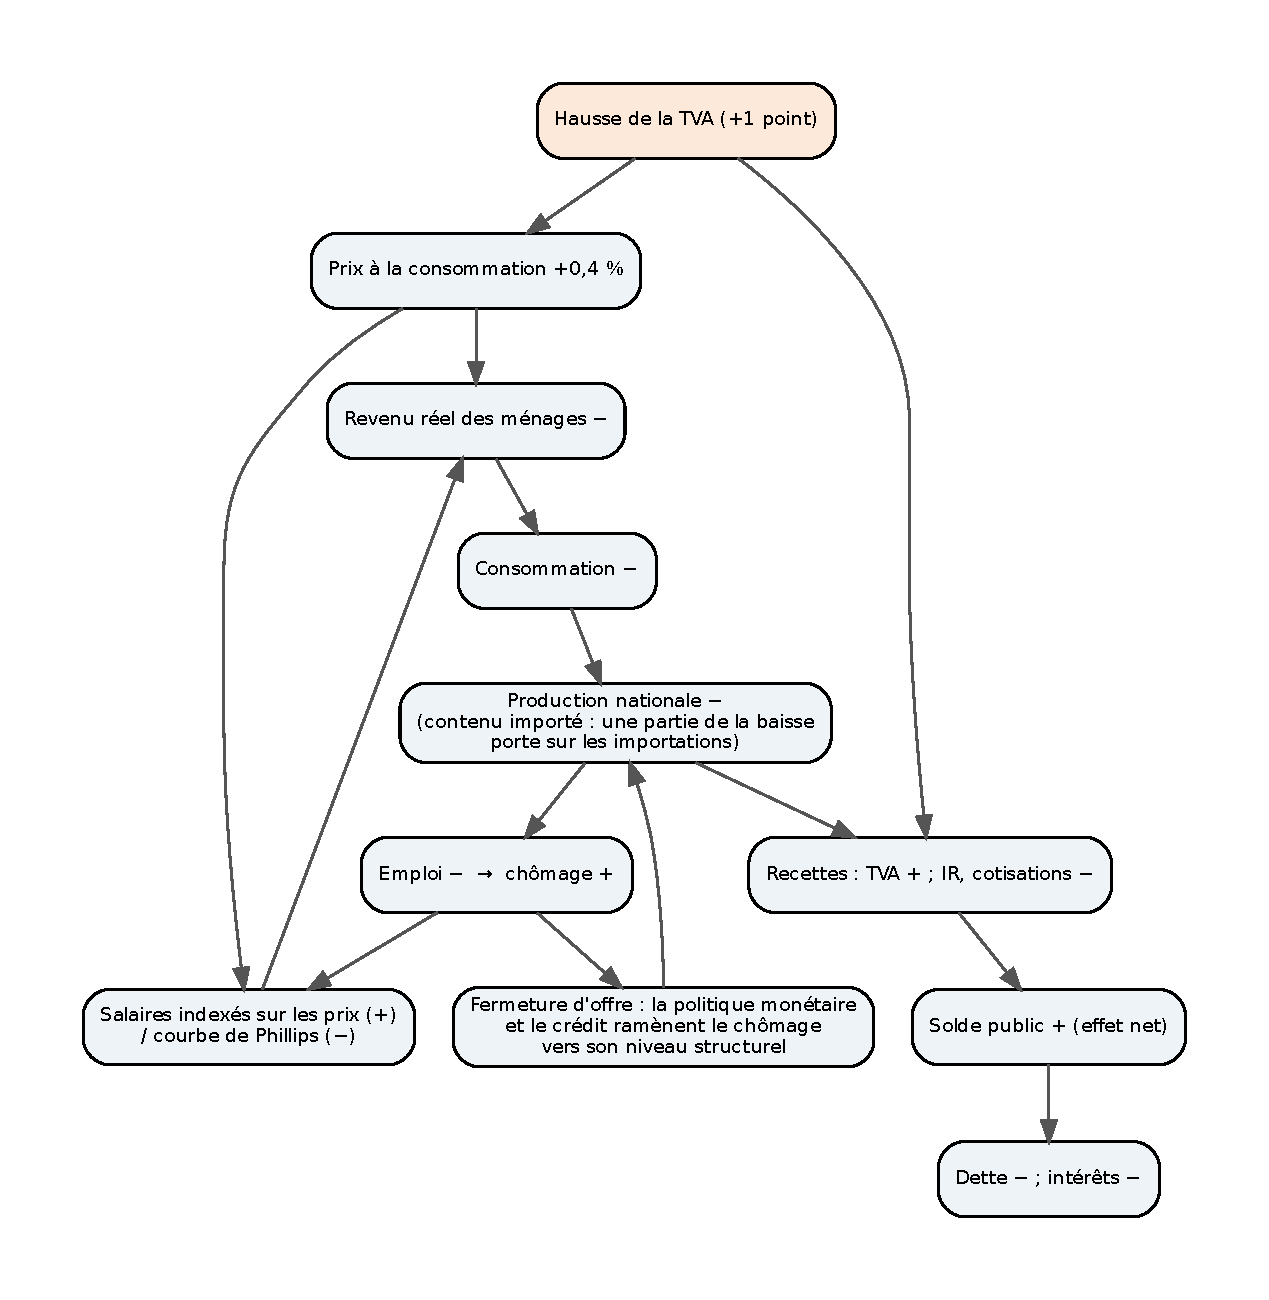
\includegraphics[width=0.78\linewidth]{chaine_causale.pdf}
\caption{Exemple de propagation : hausse d'un point du taux normal de TVA. Chaque case correspond à une ou plusieurs
équations du modèle ; les ordres de grandeur sont ceux de la simulation du chapitre~\ref{ch:experiences}.}
\label{fig:chaine}
\end{figure}

\begin{exemple}[Exemple : la propagation d'une hausse de TVA (simulation « TVA +1 point »)]
Un point de TVA rapporte statiquement environ 8,2\md{} (80~\% de la recette nette au taux normal, rapportée au taux).
Le modèle suppose qu'il est répercuté à 80~\% sur les prix : les prix à la consommation sont plus élevés de 0,42~\% en
2030. Le pouvoir d'achat des ménages baisse de 0,29~\% ; la consommation de 0,28~\%. Une partie de cette consommation
perdue portait sur des produits importés (27~\% en moyenne du contenu de la consommation) : la production nationale ne
baisse que de 0,09~\% en 2029. L'emploi recule de 23\,000 postes, le chômage monte de 0,08 point. Les
salaires, indexés en partie sur les prix, augmentent de 0,09~\%, ce qui amortit la perte de pouvoir d'achat mais
renchérit le coût du travail. Côté finances publiques, la recette nouvelle (+0,34 point de PIB de recettes) est
partiellement compensée par les moindres recettes d'impôt sur le revenu et de cotisations liées à l'activité : le
solde public s'améliore de 0,21 point de PIB en 2029, 0,24 en 2032. La dette est plus basse de 2,2 points de PIB en
2037, grâce aussi à l'effet du niveau des prix sur le PIB nominal. À long terme, la fermeture d'offre ramène l'activité
vers son niveau de référence (PIB $-$0,02~\% en 2037).
\end{exemple}

\section{Niveaux de preuve}
\label{sec:niveaux}

Chaque paramètre et chaque résultat de ce rapport est qualifié par un niveau de preuve, repris du registre des
paramètres du projet (annexe~\ref{ann:registre}) :

\begin{center}\small
\begin{tabularx}{0.95\linewidth}{@{}lL@{}}
\toprule
Code & Signification \\
\midrule
\preuve{R} & Relation comptable : vraie par définition. \\
\preuve{A} & Donnée observée (comptes nationaux, législation, statistiques publiques). \\
\preuve{E} & Coefficient estimé économétriquement sur des données françaises (avec son écart-type). \\
\preuve{C} & Calibré sur une source empirique française ou une méta-analyse. \\
\preuve{L} & Transposé de la littérature (souvent étrangère). \\
\preuve{H} & Hypothèse de modélisation, sans mesure empirique directe. \\
\bottomrule
\end{tabularx}
\end{center}

Pour les résultats, on utilise une échelle de robustesse : \fiab{robuste} (signe et ordre de grandeur stables dans
tous les tests de sensibilité), \fiab{plutôt robuste} (signe stable, ampleur variable), \fiab{fragile} (signe
dépendant d'hypothèses), \fiab{non établi} (le modèle ne permet pas de conclure).
